\let\negmedspace\undefined
\let\negthickspace\undefined
\documentclass[journal]{IEEEtran}
\usepackage[a5paper, margin=10mm, onecolumn]{geometry}
%\usepackage{lmodern} % Ensure lmodern is loaded for pdflatex
\usepackage{tfrupee} % Include tfrupee package

\setlength{\headheight}{1cm} % Set the height of the header box
\setlength{\headsep}{0mm}     % Set the distance between the header box and the top of the text
\usepackage{multicol}
\usepackage{gvv-book}
\usepackage{gvv}
\usepackage{cite}
\usepackage{amsmath,amssymb,amsfonts,amsthm}
\usepackage{algorithmic}
\usepackage{graphicx}
\usepackage{textcomp}
\usepackage{xcolor}
\usepackage{txfonts}
\usepackage{listings}
\usepackage{enumitem}
\usepackage{mathtools}
\usepackage{gensymb}
\usepackage{comment}
\usepackage[breaklinks=true]{hyperref}
\usepackage{tkz-euclide} 
\usepackage{pgfplots}
\pgfplotsset{compat=1.18}
\usepackage{listings}
% \usepackage{gvv}                                        
\def\inputGnumericTable{}                                 
\usepackage[latin1]{inputenc}                                
\usepackage{color}                                            
\usepackage{array}                                            
\usepackage{longtable}                                       
\usepackage{calc}                                             
\usepackage{multirow}                                         
\usepackage{hhline}                                           
\usepackage{ifthen}                                           
\usepackage{lscape}
\usepackage{tikz}
% Marks the beginning of the document
\begin{document}
\bibliographystyle{IEEEtran}
\vspace{3cm}

\title{Solving differential equation\\NCERT-12.9.ex.12}
\author{EE24BTECH11056 - S.Kavya Anvitha}
\maketitle
%\newpage
\bigskip

\renewcommand{\thefigure}{\theenumi}
\renewcommand{\thetable}{\theenumi}
\textbf{Question:}\\
$xdy = \brak{2x^2+1}dx$\\
\textbf{Solution:}\\
\textbf{Using Bilinear Transform technique:}\\
Original Differential Equation:
\begin{align}
    \frac{dy}{dx} = 2x + \frac{1}{x}
\end{align}
Let $\frac{dy}{dx} = x(t)$ where $x(t) = 2t + \frac{1}{t}$
Taking the Laplace transform:
\begin{align}
sY(s) = X(s)    
\end{align}
which gives the transfer function:
\begin{align}
H(s) = \frac{Y(s)}{X(s)} = \frac{1}{s}.    
\end{align}
Using the Bilinear Transform Relation\\
The bilinear transform substitutes  with a discrete-time equivalent:
\begin{align}
    s = \frac{2}{T}\left(\frac{1 - z^{-1}}{1 + z^{-1}}\right)
\end{align}
where $T$ is the sampling period. Substituting this into the equation gives :
\begin{align}
   H(z) = \frac{1}{\frac{2}{T}\left(\frac{1 - z^{-1}}{1 + z^{-1}}\right)}
\end{align}
Simplify the expression:
\begin{align}
H(z) = \frac{T}{2} \times \frac{1 + z^{-1}}{1 - z^{-1}}
\end{align}
$H(z)$ describes the transfer function in the z-domain. Rewrite it in terms of input-output relation:
\begin{align}
    H(z) = \frac{Y(z)}{X(z)}\\
\frac{Y(z)}{X(z)} = \frac{T}{2} \times \frac{1 + z^{-1}}{1 - z^{-1}}\\
\text{Cross multiply:}\\
Y(z)\left(1 - z^{-1}\right) = \frac{T}{2} X(z)\left(1 + z^{-1}\right)
\end{align}
Expanding into time domain (replace  with a delay operator):
\begin{align}
    y[n] - y[n-1] = \frac{T}{2}\left(x[n] + x[n-1]\right)
\end{align}
$x(n) = 2t(n) +\frac{1}{t(n)}$, \text{where} $t(n) = t(0) + n*h$
Substituting in the equation gives 
\begin{align}
y[n] - y[n-1] = \frac{h}{2}\brak{2t(n) +\frac{1}{t(n)} + 2t(n-1) + \frac{1}{t(n-1)}}\\
y[n] - y[n-1] = \frac{h}{2}\brak{2(t(0)+n\cdot h)+\frac{1}{t(0)+n\cdot h}+2(t(0)+(n-1) \cdot h)+ \frac{1}{t(0)+(n-1) \cdot h}}\\
\text{simplifying,}\\
y_{n} - y_{n-1} = \frac{h}{2}\brak{4t_0 + 4n\cdot h -2h + \frac{1}{t_0 + n\cdot h} + \frac{1}{t_0 + (n-1)\cdot h}}
\end{align}
here $t_0 = 1$ substituting we get 
\begin{align}
y_{n} - y_{n-1} = \frac{h}{2}\brak{4 + 4n\cdot h -2h + \frac{1}{1 + n\cdot h} + \frac{1}{1 + (n-1)\cdot h}}
\end{align}
\textbf{trapezoidal solution:}
The aim is to find the difference equation using the trapezoidal law using the following  initial conditions $x_0 = 1$ and $y_0 = 1$
\begin{align}
  \frac{dy}{dx} = 2x + \frac{1}{x}
\end{align}
1. Start with the Differential Equation\\
The given differential equation is:
\begin{align}
    \frac{dy}{dx} = f(x, y).
\end{align}
Integrate this over the interval :

\begin{align}
\int_{y_n}^{y_{n+1}} dy = \int_{x_n}^{x_{n+1}} f(x, y) \, dx\\
y_{n+1} = y_n + \int_{x_n}^{x_{n+1}} f(x, y) \, dx.
\end{align}
3. Generalize Over Multiple Intervals

Now, consider the integral over multiple intervals from  to :
\begin{align}
\int_{x_0}^{x_n} f(x) \, dx.
\end{align}
Using the trapezoidal rule, we approximate this integral as:
\begin{align}
\int_{x_0}^{x_n} f(x) \, dx \approx \frac{h}{2} \left[ f(x_0) + 2f(x_1) + 2f(x_2) + \cdots + 2f(x_{n-1}) + f(x_n) \right].
\end{align}
This can be expressed as:
\begin{align}
\int_{x_0}^{x_n} f(x) \, dx \approx h \left[ \frac{1}{2} f(x_0) + f(x_1) + f(x_2) + \cdots + f(x_{n-1}) + \frac{1}{2} f(x_n) \right].
\end{align}

The trapezoidal rule approximates an integral over an interval  as:
\begin{align}
\int_{x_n}^{x_{n+1}} f(x) \, dx \approx \frac{h}{2} \left[ f(x_n) + f(x_{n+1}) \right],
\end{align}
4. Substitute Back into the Differential Equation

Returning to the differential equation, , the difference equation becomes:
\begin{align}
y_{n+1} = y_n + \frac{h}{2} \left[ f(x_n, y_n) + f(x_{n+1}, y_{n+1}) \right].
\end{align}
The function  is:
\begin{align}
f(x, y) =  2x + \frac{1}{x}.
\end{align}
Substitute  and  into the general trapezoidal formula:
\begin{align}
y_{n+1} = y_n + \frac{h}{2} \left[2x_n + \frac{1}{x_n} + 2x_{n+1} +\frac{1}{x_{n+1}} \right].
\end{align}
 Express $x_{n+1}$ Explicitly \\
 since 
 \begin{align}
     x_{n+1} = x_n + h,
 \end{align}
 substitute this into the second term: 
 \begin{align}
     2x_{n+1} + \frac{1}{x_{n+1}} = 2(x_n + h) + \frac{1}{x_n + h}.
 \end{align}
 Now rewrite the formula:
 \begin{align}
     y_{n+1} = y_n + \frac{h}{2} \left[2x_n +  \frac{1}{x_n} + 2(x_n + h) + \frac{1}{x_n + h} \right].
     y_{n+1} = y_n + \frac{h}{2} \brak{4x_n + 2h + \frac{1}{x_n}+\frac{1}{x_n + h}}
 \end{align}
 \textbf{theoretical solution:}
 \begin{align}
    \frac{dy}{dx} = 2x + \frac{1}{x}\\
    dy = \brak{2x+\frac{1}{x}}dx\\
    \int dy = \int\brak{2x+\frac{1}{x}}dx\\
    y = x^2 + \log{\abs{x}} + C
\end{align}
given it passes through \myvec{1,1} C = 0
Therefore: 
\begin{align}
    y = x^2 + \log{\abs{x}}
\end{align}
 \begin{figure}[h!]
   \centering
   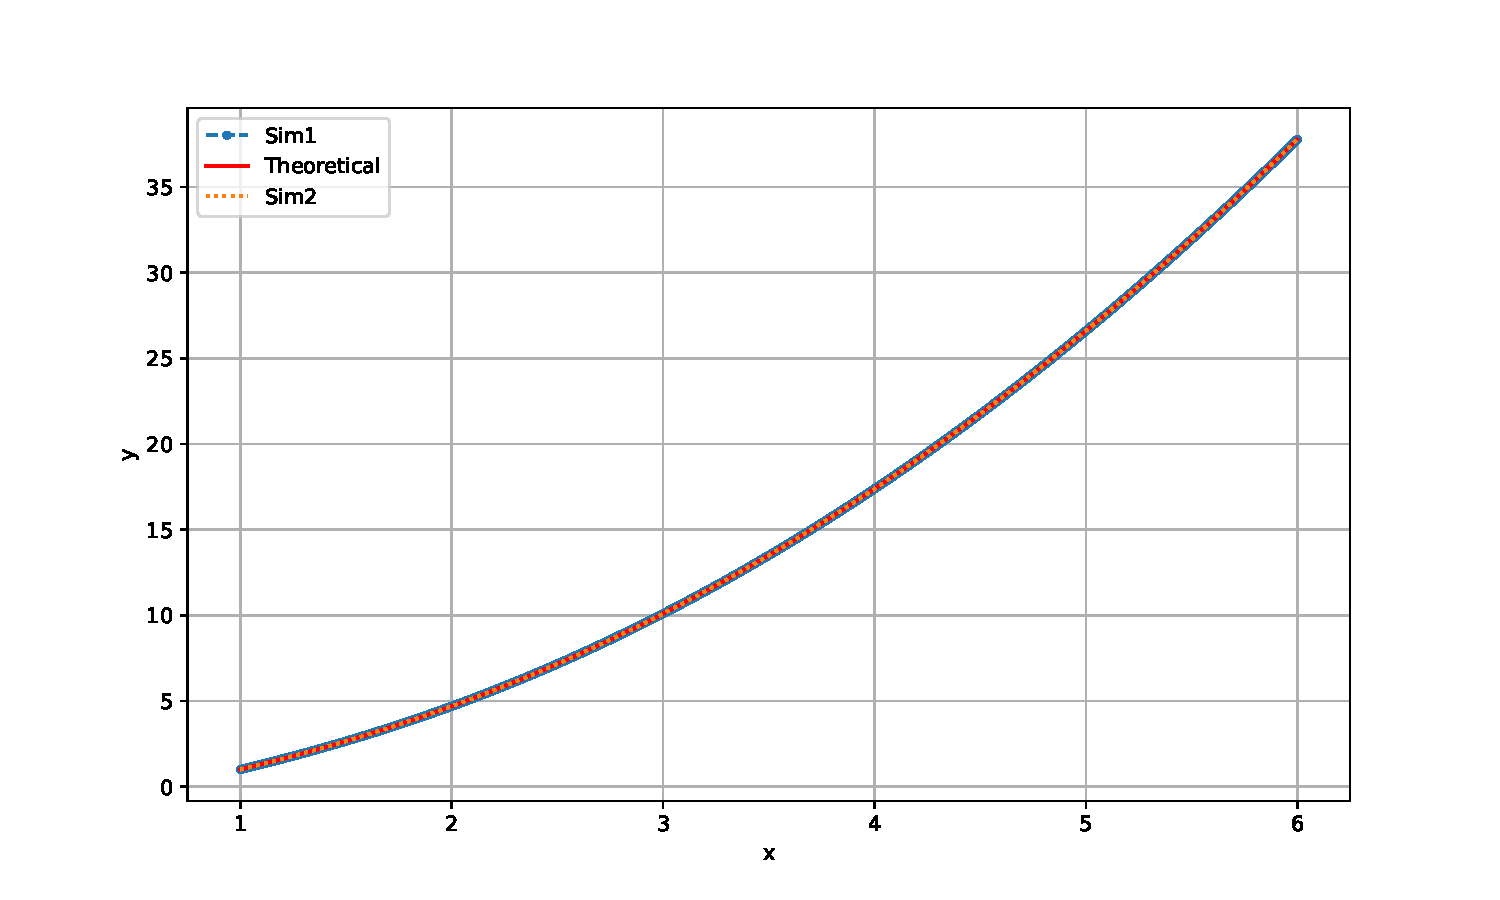
\includegraphics[width=\columnwidth]{figs/fig.pdf}
\end{figure}
\end{document}
